% !TEX root = ../team-report.tex
% ERA-Großpraktikum: Team Bericht -- Gruppendynamik (Slack)

\subsection{Slack}
\label{team:group-slack}

Unser wichtigster Kommunikationskanal war die Teamchat-Software \emph{Slack}.
Slack erlaubt sowohl persönliche, "vier-Augen" Chats, als auch die Aufspaltung
der Diskussion in themenspezifische \emph{Kanäle} (engl. \emph{Channels}). Bei
der Entwicklung von \erasim{} verteilten wir unsere Kommunikation hierbei auf
zwei Arten von Kanälen: \emph{Teamkanäle} und \emph{Topic-Kanäle}.

Teamkanäle waren jene Kanäle, in denen jede Untergruppe von \erasim{}, also
\emph{Arch, Core, Parser} und \emph{GUI}, Diskussionen führen konnten, die sich
rein mit den Aspekten der Entwicklung von \erasim{} befassten, die jeder Gruppe
entsprachen. In diesen Chats wurde über den Fortschritt sowie aufgetretene
Probleme eines einzelnen Mitglieds der Untergruppe berichtet, wichtige
Informationen zur Entwicklungsumgebung diskutiert (z.B. eine neue Qt Version
oder die Veröffentlichung einer neuen RISC-V Spezifikation) oder auf scheiternde
Tests aufmerksam gemacht. Wichtig hierbei war insbesondere, dass diese Teamchats
nicht für die Untergruppe privat, sondern für das ganze \erasim{} Team
öffentlich war. Somit konnten auch von Mitgliedern anderer Untergruppen Fragen
gestellt bzw. wichtige Entwicklungen mitgeteilt werden. Wollte beispielsweise
ein Mitglied des Core wissen, auf welchem Wege man am besten die Registergröße der
momentan geladenen Architektur abruft, so konnte er oder sie diese Frage im
Arch-Chat stellen und ihm oder ihr wurde meist auch schnell geholfen.

Neben Teamkanälen wurde auch kräftig in den Topickanälen diskutiert. Ein
Topickanal beschränkte sich auf ein spezifisches Gebiet der Entwicklung oder
anderen Themen. Ein wichtiger und vielgenutzter Kanal war beispielsweise der
C\texttt{++} Channel. In diesem konnten Fragen zu C++ gestellt, stilistische
Aspekte des Google Style Guides diskutiert oder auch bezüglich kryptischen
Kompilierfehlern nachgefragt werden. Mitglieder mit mehr C++ Erfahrung konnten
diese Fragen dann beantworten oder auf entsprechende Ressourcen hinweisen. Ein
anderer Topickanal war \emph{report} genannt, in welchem die Planung und
Fertigstellung des ersten und finalen Berichts besprochen wurde. Ein weiteres
nützliches Feature von Slack ist die Integration mit externen Dienstleistungen.
So gab es einen weiteren Topickanal, genannt \emph{notifications}, in welchen
wir unseren Test-Server \emph{Travis} integriert hatten. Immer wenn unsere Tests
auf Travis scheiterten oder erfolgreich waren, erhielten wir in diesem Kanal
eine Benachrichtigung. Dadurch musste man auch nicht mehr die Website von Travis
besuchen, um den Status der Tests zu erfahren.

In Summe waren gegen Ende der Entwicklung auf Slack 12 Kanäle offen --- 4
Teamkanäle und 8 Topickanäle. In diesen Kanälen und über private Chats wurden
über den gesamten Entwicklungszeitraum hinweg gesammelt 14,800 Nachrichten
ausgetauscht. \autoref{fig:slack} schlüsselt diese Zahl weiter auf.

\begin{figure}[h!]
  \centering
  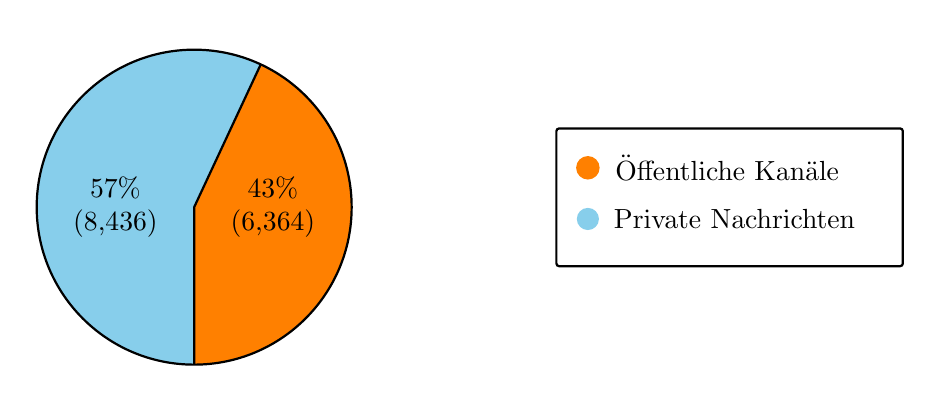
\begin{tikzpicture}[thick]

    % Public Channels
    \fill [SkyBlue]
          (0, -2) -- (0, 0) -- (65:2cm)
          arc [radius=2cm, start angle=65, end angle=270];

    % Direct Messages
    \fill [orange]
          (0, -2) -- (0, 0) -- (65:2cm)
          arc [radius=2cm, start angle=65, end angle=-90];

    % Pie border
    \draw (0, 0) circle [radius=2cm];

    % Sector border
    \draw (0, -2) -- (0, 0) -- (65:2cm);

    % Labels
    \node at (-1, 0) [align=center] {57\% \\ (8,436)};
    \node at (+1, 0) [align=center] {43\% \\ (6,364)};

    % Legend
    \path (5, 0.5) coordinate [fill, orange, circle, inner sep=3pt] (public)
          node [right] {\hspace{0.1cm} Öffentliche Kanäle};
    \fill [SkyBlue] (public)+(0, -0.65cm) circle [radius=4pt]
          node [right] {\hspace{0.2cm}\color{black} Private Nachrichten};
    \draw [thick, rounded corners=1pt]
          (public)+(-0.4, +0.5) rectangle ++(4, -1.25);

  \end{tikzpicture}
  \caption{Eine Aufschlüsselung der über Slack versendeten
  Nachrichten. Der relative Anteil und die absolute Anzahl an Nachrichten in
  öffentlichen Kanälen sind in Orange eingezeichnet, private Nachrichten in
  Türkis. Insgesamt wurden über 10 Monate hinweg 14,800 Nachrichten verschickt.}
  \label{fig:slack}
\end{figure}

\vspace{-0.5cm}
